\chapter{Napadi}

\newcommand{\norm}[1]{\left\|{#1}\right\|}

\section{Uvod}

Neprijateljski napad je tehnika korištenja neprijateljskih primjera s ciljem manipulacije izlaza klasifikacijskog modela. Neprijateljski primjer je neprimjetno izmijenjena originialna slika koju klaisifikacijski model zbog izmjena više ne klasificira ispravno.

Na primjer, kod modela za prepoznavanje znamenki, ulazna slika koju model inače (točno) klasificira kao broj ‘9’ se može neprimjetno izmijeniti i krivo klasificirati kao broj ‘4’ (Slika \ref{fig:example}).

\begin{figure}[H]
    \centering
    \subfloat[\centering Originalna slika]{{
\includegraphics[width=4.5cm]{slike/napadi/uvod-example.png} }}%
    \qquad
    \subfloat[\centering Perturbirana slika]{{
\includegraphics[width=4.5cm]{slike/napadi/uvod-example-w-eps.png} }}%
    \caption{Primjer neprijateljskog napada, $\epsilon = 0.2$}%
    \label{fig:example}%
\end{figure}

\section{Sažetak} 

Za izgradnju neprijateljskog primjera, koristimo metodu FGSM (engl. \textit{Fast Gradient Sign Method}). Ta metoda uključuje izračun gradijenata te njihovu primjenu na ulazne podatke, ali u smjeru najbržeg rasta funkcije gubitka. Na taj način dobivamo suprotan efekt učenju modela (a to je smanjenje funkcije gubitka i bolja klasifikacija) te udaljujemo izlazne vrijednosti od onih očekivanih. Metodu primjenjujemo na način da ulazne podatke (u našem slučaju vrijednosti piksela slike) tretiramo kao parametre modela kako bi i za njih izračunali gradijente. \\

Koristimo tri različita napada na model za pogrešnu klasifikaciju slike: 
\begin{itemize}
    \item Promjena piksela slike za jednaku vrijednost u smjeru predznaka gradijenata
    \item Promjena piksela slike u smjeru predznaka gradijenta izračunatog nad ciljnom klasom
    \item Promjena nekog udjela piksela kojima pripadaju najznačajniji gradijenti za jednaku vrijednost
\end{itemize}

\section{FGSM napad}

FGSM (engl. \textit{Fast Gradient Sign Method}) je vrsta neprijateljskog napada koji se bazira na dodatku linearne količine šuma slici u smjeru predznaka gradijenta $\nabla J(x, y, \theta)$. Gdje $J$ predstavlja funkciju gubitka. Izračun gradijenata slike se može provesti nastavkom običnog gradijentnog spusta "jedan korak dalje" na samu sliku, što efektivno tretira ulaz kao parametre modela. Kao i inače, dobiveni gradijenti predstavljaju smjer izmjene za (lokalnu) maksimizaciju funkcije gubitka. Ukoliko perturbaciju označimo sa $\eta$, neprijateljski primjer se može zapisati kao: 
\[\widetilde{x} = x + \eta\]

Glavna ideja FGSM napada je pretpostavka da možemo pronaći dovoljno mali $\eta$ koji znatno utječe na izlaz modela, dok je ljudskom oku promjena neprimjetna. Iako je gradijent $\nabla J(x, y, \theta)$ po definiciji smjer najvećeg porasta gubitka (odnosno ono što želimo postići), da bi osigurali gornju granicu za $\eta$, ne možemo postaviti $\eta = \nabla J(x, y, \theta)$. Zbog toga, za $\eta$ uzimamo vrijednost: 
\[\eta = \epsilon \cdot sign\left(\nabla J(x, y, \theta)\right)\]

To osigurava ispunjenje uvjeta $\epsilon \geq \norm{\eta}$. Vrijednost $\epsilon$ je proizvoljna, čime možemo kontrolirati količinu šuma korištenog za perturbaciju. Perturbirana slika se sada može prikazati formulom: 
\[\widetilde{x} = x + \epsilon\cdot sign\left(\nabla J(x, y, \theta)\right)\]

U kodu to izgleda ovako:

\textbf{L53 u neprijateljski\_primjer\_funkcije.py ovdje}

\section{FGSM napad s ciljnom klasom}

Malom izmjenom FGSM napada možemo dobiti neprijateljski napad s ciljnom klasom. Cilj ovog napada je izmijeniti sliku na takav način da ju model klasificira kao neku unaprijed odabranu klasu različitu od originalne. To se postiže promjenom načina računanja gubitka i smjera perturbacije slike. Za izračun gubitka se koristi ciljna klasa umjesto prave labele, dok se prava labela primjera potpuno zanemaruje.  Zbog toga, minimizacijom gubitka također maksimiziramo vrijednost predikcije za našu ciljnu klasu. Cilj običnog FGSM napada je maksimizirati gubitak, stoga naša varijanta također zahtijeva i promjenu smjera u formuli perturbacije slike. Kao i prije, korak se provodi samo za ulaz, dok težine modela ostaju fiksne. Perturbirana slika se sada može prikazati formulom: 
\[\widetilde{x} = x - \epsilon\cdot sign\left(\nabla J(x, y_c, \theta)\right)\]

Gdje $y_c$ predstavlja ciljnu klasu. U kodu to izgleda ovako:

\textbf{L98 u neprijateljski\_primjer\_funkcije.py ovdje}

\section{FGSM napad s najznačajnijim pikselima}

Ideja iza ovog napada je odabir onih piksela koji najviše utječu na promjenu funkcije gubitka. Na taj način možemo odabrati dio svih piksela tako da slika izgleda manje promijenjeno, a svejedno prevariti model. \\
U ovom napadu, osim parametra $\epsilon$ imamo i parametar $p$ koji predstavlja udio promijenjenih komponenti piksela. Budući da su pikseli naših podataka dani odvojeno po RGB komponentama te za svaku računamo vlastite gradijente, mi mijenjamo te komponente zasebno umjesto cijele piksele. Posljedično ćemo promijeniti vrijednosti više piksela, ali nećemo svakom pikselu promijeniti sve komponente. U kodu to izgleda ovako:
\begin{minted}{python}
grads = image.grad.reshape(-1,) # 1x3xAxB u 1*3*A*B
abs_grads = torch.abs(grads)
k = int(abs_grads.numel() * p)
kth_biggest_grad = abs_grads.kthvalue(
abs_grads.numel() - k).values.item()
selected_grads = abs_grads.gt(
kth_biggest_grad).int().reshape(image.shape)

# Perturbiramo sliku
new_image = image + eps * image.grad.sign() * selected_grads
\end{minted}

Pregled rezultata s različitim $\epsilon$ i $p$, elementi u tablici označavaju udio slika koje je model ispravno klasificirao nakon izmjene (model za slike bez izmjene ima točnost od oko 87\%):

\begin{table}[H]
	\centering
	\begin{tabular}{||c || c c c||} 
		\hline
		$\epsilon \backslash p$ & 0.1 & 0.25 & 0.5 \\ [0.5ex] 
		\hline\hline
		0.1 & 38\% & 18\% & 10\% \\ 
		0.25 & 23\% & 8\% & 4\% \\
		0.5 & 20\% & 8\% & 6\% \\ [1ex] 
		\hline
	\end{tabular}
	\caption{Prikaz ispravnosti modela za napad s najznačajnijim pikselima}
\end{table}

Možemo primijetiti da povećanjem parametara $\epsilon$ i $p$ točnost modela pada. Također, povećanje parametra p puno više utječe na točnost od parametra $\epsilon$. Primjer krivo klasificirane slike kada su oba parametra 0.1:
\begin{figure}[H]
	\centering
	{{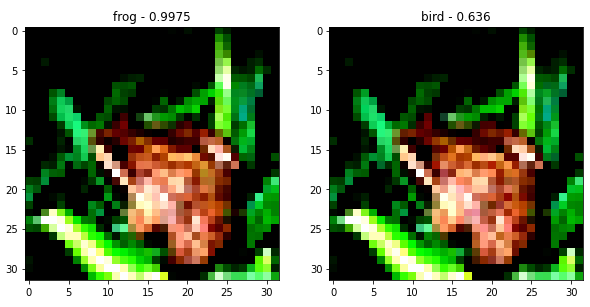
\includegraphics[width=12cm]{slike/napadi/selected-grads-example.png} }}%
	\caption{Prikaz točno kvalificirane (lijevo) i netočno kvalificirane slike (desno), $\epsilon = p = 0.1$}%
	\label{fig:example}%
\end{figure}

Prikažimo $5\%$ najznačajnijih gradijenata za prethodnu sliku. Bojom piksela možemo prikazati koje se komponente tog piksela nalaze u $5\%$ najznačajnijih gradijenata. Ako neki piksel sadrži određenu komponentu, onda je ona dio tih gradijenata.
\begin{figure}[H]
	\centering
	{{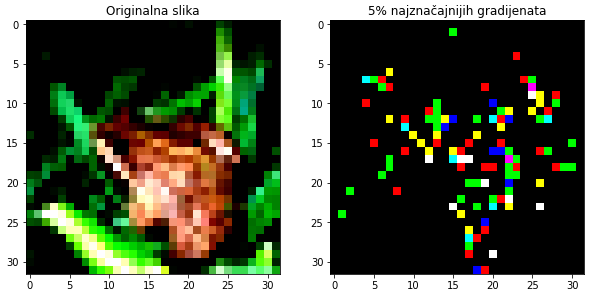
\includegraphics[width=12cm]{slike/napadi/selected-grads-visualisation.png} }}%
	\caption{Prikaz $5\%$ najznačajnijih gradijenata}%
	\label{fig:example}%
\end{figure}

\section{Rezultati}

Usporedimo rezultate različitih napada s različitim parametrima $\epsilon$. \\

Za prethodno navedene napade i tri različite $\epsilon$ vrijednosti prikažimo udio izmijenjenih slika koje model klasificira u njihovu pravu klasu. Prvi napad je običan FGSM napad, drugi je FGSM napad s ciljnom klasom, a treći je FGSM napad s najznačajnijim pikselima u kojem uzimamo $p = 0.25$. Model za slike bez izmjene ima točnost od oko 87\%.

\begin{table}[H]
	\centering
	\begin{tabular}{||c || c | c | c||} 
		\hline
		$\epsilon$ & Napad 1 & Napad 2 & Napad 3 \\ [0.5ex] 
		\hline\hline
		0.01 & 71\% & 86\% & 79\% \\ 
		0.1 & 5\% & 25\% & 18\% \\
		0.25 & 3\% & 14\% & 8\% \\ [1ex] 
		\hline
	\end{tabular}
	\caption{Usporedba ispravnosti modela za razne napade}
\end{table}

Vidimo da ni jedan napad nije jako učinkovit za $\epsilon = 0.01$. Za veće $\epsilon$ najučinkovitiji je običan FGSM napad. To je i za očekivati jer treći napad, FGSM s najznačajnijim pikselima, mijenja količinski četiri puta manje vrijednosti od običnog FGSM napada dok im je $\epsilon$ zajednički. Najlošiji napad je FGSM s ciljnom klasom, no on ne mijenja sliku u smjeru gradijenata funkcije gubitka, već u određenom smjeru koji je manje učinkovit.